\documentclass[journal]{IEEEtran}

\usepackage[utf8]{inputenc}
\usepackage[T1]{fontenc}
\usepackage{amsmath,amssymb,amsfonts}
\usepackage{graphicx}
\usepackage{booktabs}
\usepackage{array}
\usepackage{url}
\usepackage[hidelinks]{hyperref}
\usepackage{orcidlink}
\graphicspath{{../figures/}}

% IEEEtran hard-codes an em-dash after the abstract and index-terms names; the CAOS
% content standard (ADR-0067) excludes em-dashes, so the separator is a full stop.
\makeatletter
\def\abstract{\normalfont
    \if@twocolumn
      \@IEEEabskeysecsize\bfseries\textit{\abstractname}.\ \relax
    \else
      \bgroup\par\addvspace{0.5\baselineskip}\centering\vspace{-1.78ex}\@IEEEabskeysecsize\textbf{\abstractname}\par\addvspace{0.5\baselineskip}\egroup\quotation\@IEEEabskeysecsize
    \fi\@IEEEgobbleleadPARNLSP}
\def\IEEEkeywords{\normalfont
    \if@twocolumn
      \@IEEEabskeysecsize\bfseries\textit{\IEEEkeywordsname}.\ \relax
    \else
      \bgroup\par\addvspace{0.5\baselineskip}\centering\@IEEEabskeysecsize\textbf{\IEEEkeywordsname}\par\addvspace{0.5\baselineskip}\egroup\quotation\@IEEEabskeysecsize
    \fi\@IEEEgobbleleadPARNLSP}
\makeatother

% Page-1 header block (conventions/manuscript-header-standard.md). The four document
% macros are set by the publishing tool when the version DOI is reserved.
\newcommand{\doctype}{Preprint}
\newcommand{\docversion}{v2.2}
\newcommand{\docdate}{18 September 2026}
\newcommand{\versiondoi}{10.5281/zenodo.22822861}
\newcommand{\conceptdoi}{10.5281/zenodo.21508920}
\newcommand{\docrepo}{github.com/fsantibanezleal/CAOS\_RES\_ChronoScope}
\newcommand{\headerblock}{%
\begin{center}
\fbox{\parbox{0.94\textwidth}{\small\raggedright
\textbf{\doctype} \quad$\cdot$\quad \docversion, \docdate \quad$\cdot$\quad Licence CC BY 4.0\\[2pt]
CAOS open-research programme \quad$\cdot$\quad CAOS\_RES\_ChronoScope, time-series forecasting method atlas\\[2pt]
Version DOI \href{https://doi.org/\versiondoi}{\texttt{\versiondoi}} \quad$\cdot$\quad
concept DOI (always latest) \href{https://doi.org/\conceptdoi}{\texttt{\conceptdoi}}\\[2pt]
Not peer reviewed. Source code, data and computational records: \href{https://\docrepo}{\texttt{\docrepo}}
}}
\end{center}}

\begin{document}

\title{Prequential Streaming Evaluation of Stateful Time-Series Forecasters with
Online Conformal Calibration: A Diagnostic Atlas and the \texttt{preqts} Harness}

\author{%
  Felipe Santib\'a\~nez-Leal~\orcidlink{0000-0002-0150-3246},~\IEEEmembership{Independent Researcher}%
  \thanks{F.\ Santib\'a\~nez-Leal is with the CAOS open-research programme, Santiago,
    Chile (e-mail: \texttt{fsantibanezleal@ug.uchile.cl}; ORCID: 0000-0002-0150-3246).}%
  \thanks{The harness is released as the open-source package \texttt{preqts}
    (\url{https://pypi.org/project/preqts/}); the atlas (code, per-case artifacts,
    workbench) is at \url{https://github.com/fsantibanezleal/CAOS_RES_ChronoScope} (MIT),
    and an interactive workbench is available at \url{https://chronoscope.fasl-work.com}.}%
}

\markboth{\doctype\ \docversion, 2026 \textperiodcentered\ CAOS open-research programme}{Santib\'a\~nez-Leal:
Prequential Streaming Evaluation of Stateful Forecasters with Online Conformal Calibration}

\IEEEaftertitletext{\vspace{-0.6\baselineskip}\headerblock\vspace{0.2\baselineskip}}

\IEEEtitleabstractindextext{%
\begin{abstract}
Real forecasting is streaming: observations arrive one by one, the model updates, and its
prediction intervals must stay calibrated as the series drifts. Yet every widely used
forecasting benchmark harness evaluates models statelessly on rolling windows, carrying no
state across windows and never running a test-then-train loop. We address this gap
with a prequential streaming evaluation harness for \emph{stateful} forecasters, released as
the open-source package \texttt{preqts}: it implements Dawid's predict-then-observe-then-update
protocol behind a \texttt{StatefulForecaster} interface with an explicit covariate-arrival
policy, and records four trajectories per method, rolling scaled error, rolling empirical
coverage, the rolling weighted quantile loss (a quantile-based probabilistic score), and cumulative compute cost, the
last of which separates a stateful constant-cost model from a replay-everything wrapper. The
harness is embedded in an
atlas that first \emph{understands} each series with ten diagnostic families (stationarity,
autocorrelation, seasonality, filters, change points, volatility, distribution and complexity,
fractal structure, nonlinear dynamics, and cross-series causality) and then forecasts it with a
nineteen-method ladder (classical, statistical, gradient-boosted, deep, and stateful foundation
models), so that the diagnosis explains the no-free-lunch leaderboard. Using the harness we test
a concrete claim: that online conformal calibration keeps streaming intervals at nominal under
distribution shift. On fifteen series that span distinct regimes and include white-noise and
random-walk negative controls, wrapping a Theta point forecaster in Adaptive Conformal Inference
or Conformal-PID control reduces the mean absolute coverage error at the nominal $80\%$ level
from $0.042$ (raw Theta) and $0.060$ (seasonal-naive) to $0.0057$ and $0.0060$, a seven-to-tenfold
reduction, and shrinks the across-case span of the final coverage from $0.19$--$0.40$ to $0.04$,
without changing the point forecast. The calibration holds on the negative controls, where a
spurious skill gap would flag harness leakage. The contribution is the reusable stateful-streaming
harness, evaluated under the protocol forecasters are actually deployed under, and a
leakage-guarded, reproducible demonstration of where online conformal calibration earns its keep.
\end{abstract}

\begin{IEEEkeywords}
time-series forecasting, prequential evaluation, streaming, conformal prediction, adaptive
conformal inference, calibration, coverage, stateful forecasters, foundation models,
diagnostics, benchmark, reproducibility.
\end{IEEEkeywords}}

\maketitle
\IEEEdisplaynotcompsoctitleabstractindextext
\IEEEpeerreviewmaketitle

% =====================================================================
\section{Introduction}
% =====================================================================

\IEEEPARstart{F}{orecasting} in production is a streaming problem: a datum arrives, the model
issues a prediction for the next horizon, the truth is later revealed, and the model updates
its state before the next step; the prediction interval must remain calibrated throughout, even
as the series drifts across regimes. This is not how forecasting models are usually evaluated.
The widely used harnesses, including the rolling-window backtests of GluonTS and Darts and the
window-based fev-bench~\cite{shchur2025}, score forecasters \emph{statelessly}: each window is
independent, no learned state carries across windows, and there is no test-then-train loop. None
of these harnesses evaluates a \emph{stateful} streaming forecaster
prequentially with an explicit policy for when covariates arrive.

We fill it with \texttt{preqts}, an open-source harness implementing the prequential principle,
Dawid's ``predictive sequential'' test-then-train protocol~\cite{dawid1984}: at each step the
model predicts, the truth is revealed and scored, and only then does the model update. Skill
becomes a trajectory over the stream rather than a single number. The harness is embedded in an
atlas (Section~\ref{sec:atlas}) that pairs the forecast with a diagnostic layer, so that the
character of a series explains why one method family wins and another fails, the no-free-lunch
principle, made legible. We then use the harness to answer a specific question
(Section~\ref{sec:results}): does online conformal calibration keep streaming intervals
calibrated under distribution shift? Our contributions are: (i) the reusable prequential
streaming harness \texttt{preqts} for stateful forecasters with a covariate-arrival policy;
(ii) a reproducible, control-guarded demonstration that online conformal calibration
reduces streaming coverage error seven-to-tenfold and collapses its across-case spread, without
changing the point forecast.

% =====================================================================
\section{The atlas: understand, then forecast}
\label{sec:atlas}
% =====================================================================

ChronoScope pairs a diagnostic layer with a forecast ladder over fifteen cases, each
computed deterministically (an artifact is a pure function of case and seed). \textbf{Ten
diagnostic families} characterize a series before it is forecast: stationarity and unit roots
(ADF, KPSS, Phillips--Perron, DF-GLS, Zivot--Andrews); autocorrelation (ACF/PACF, Ljung--Box);
seasonality (periodogram, STL/MSTL, seasonal strength); filters and adaptive decompositions
(Hodrick--Prescott, Baxter--King, EMD/CEEMDAN, wavelet scalogram); change points and regimes
(PELT, OLS-CUSUM, Hamilton Markov-switching); volatility and transforms (ARCH-LM, GARCH,
Box--Cox); distribution, normality and complexity (moments, Jarque--Bera, sample/spectral
entropy, the BDS test, and the catch22 feature set~\cite{lubba2019}); fractal and multifractal
structure (Hurst via R/S and DFA, MF-DFA, ARFIMA long memory); nonlinear dynamics and chaos
(Takens embedding, largest Lyapunov exponent, recurrence quantification, the 0--1 test, with a
surrogate-data test for nonlinearity); and cross-series causality (cross-correlation lead/lag,
Granger, Engle--Granger and Johansen cointegration). Each is a verified implementation wrapped in
a NaN-safe API and precomputed per case.

\textbf{A nineteen-method forecast ladder} is then scored on the same cases: classical
numpy live methods (seasonal-naive, SES, Holt, Holt--Winters, Theta~\cite{assimakopoulos2000}),
statistical methods (AutoARIMA, AutoETS, AutoTheta), a gradient-boosted method (LightGBM), deep
methods, and stateful zero-shot foundation models (Chronos~\cite{ansari2024},
TimesFM~\cite{das2024}). The cases span distinct regimes by construction, level shift,
deterministic chaos, GARCH heteroskedasticity, intermittent demand, long memory, coupled
daily/weekly seasonality, exogenous promotions, plus real CC-BY series (UCI Electricity, Beijing
PM2.5, M4 excerpts~\cite{makridakis2020}) and two negative controls, white noise and a near-random walk. There is no
universal winner: the diagnosis explains the leaderboard, which is exactly the setting in which
leakage-free scoring matters most.

% =====================================================================
\section{The prequential streaming harness}
\label{sec:harness}
% =====================================================================

\begin{figure*}[!t]
\centering
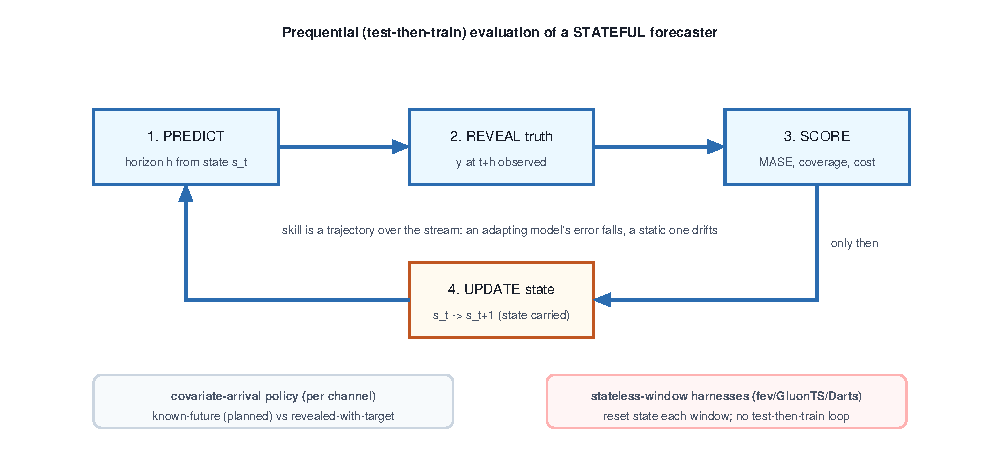
\includegraphics[width=0.9\textwidth]{fig-prequential.pdf}
\caption{The prequential test-then-train loop for a stateful forecaster. At each step the model
predicts from its current state, the truth is revealed and scored, and only then is the state
updated; a covariate-arrival policy declares, per channel, whether a value is known at prediction
time or revealed with the target. Stateless-window harnesses reset state each window and run no
test-then-train loop, so they cannot see a calibrator recover coverage after a shift.}
\label{fig:prequential}
\end{figure*}

Let a stream deliver observations $y_1,y_2,\dots$ At step $t$ a stateful forecaster $f$ with state
$s_t$ issues a horizon-$h$ prediction and an interval at nominal level $1-\alpha$; the truth
$y_{t+h}$ is then revealed, the prediction scored, and the state updated (Fig.~\ref{fig:prequential}),
\begin{equation}
(\hat y_{t+h},\hat I_t)=f_\text{predict}(s_t),\qquad s_{t+1}=f_\text{update}(s_t,y_{t+h}).
\end{equation}
The update strictly follows scoring, so no point is used to predict itself; a covariate-arrival
policy declares, per exogenous channel, whether its value at $t+h$ is known at prediction time (a
planned promotion) or revealed with the target (a realized driver). After a warmup the harness
records, as functions of stream position, four trajectories: the rolling scaled error, the rolling
empirical coverage, the rolling weighted quantile loss, and the cumulative compute cost, the constant-cost-per-step
signature that separates a stateful model from a replay-everything wrapper. Point accuracy uses the
mean absolute scaled error (MASE)~\cite{hyndman2006}; interval quality is read two ways that cannot
be gamed independently, empirical coverage versus the nominal level, and the weighted quantile loss
(WQL), the quantile (pinball) loss summed over the levels $0.1$, $0.5$ and $0.9$ and normalized by
the sum of absolute target values, which penalizes both interval width and misses. The quantile
loss is a proper scoring rule for quantile forecasts~\cite{gneiting2007}, and its average over
quantile levels approximates the continuous ranked probability score (CRPS)~\cite{ansari2024}. The
harness sits behind a
\texttt{StatefulForecaster} interface so classical methods, gradient-boosted models, and stateful
foundation models are evaluated identically, and it is published as the package \texttt{preqts};
because the streaming artifact carries only aggregate metric trajectories (no raw series values are
recoverable), the demonstration can be released even for real datasets licensed for local use only.

% =====================================================================
\section{Online conformal calibration}
\label{sec:conformal}
% =====================================================================

Split-conformal prediction issues an interval whose width is a quantile of past nonconformity
scores (here absolute residuals); under exchangeability its coverage is $1-\alpha$. Streams are
not exchangeable, so the effective level must adapt. \textbf{Adaptive Conformal
Inference}~\cite{gibbs2021} updates the level each step by the observed miss,
\begin{equation}
\alpha_{t+1}=\alpha_t+\gamma\,(\alpha-\text{err}_t),\qquad \text{err}_t=\mathbf 1\{y_{t+h}\notin\hat I_t\},
\label{eq:aci}
\end{equation}
so long-run coverage converges to the target under arbitrary distribution shift.
\textbf{Conformal-PID control}~\cite{angelopoulos2023} generalizes this to a
proportional-integral-derivative controller on the coverage error, with ACI as the integral-only
special case; the proportional and derivative terms buy faster coverage recovery after a regime
change. Both wrap any point forecaster and change only the interval, never the point prediction.

% =====================================================================
\section{Results}
\label{sec:results}
% =====================================================================

\begin{figure}[!t]
\centering
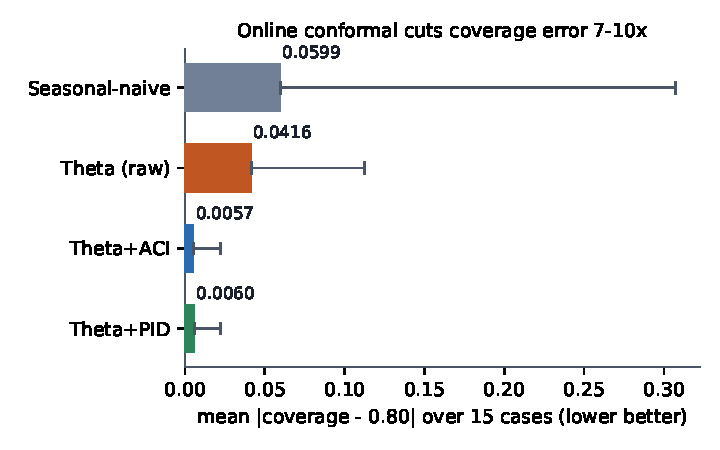
\includegraphics[width=\columnwidth]{fig-coverage-summary.pdf}
\caption{Mean absolute coverage error at nominal $80\%$ over the fifteen cases (bar) with the
worst-case per-case error (whisker). Online conformal cuts the error seven-to-tenfold. Data: the
per-case \texttt{streaming.json} artifacts.}
\label{fig:summary}
\end{figure}

\begin{figure}[!t]
\centering
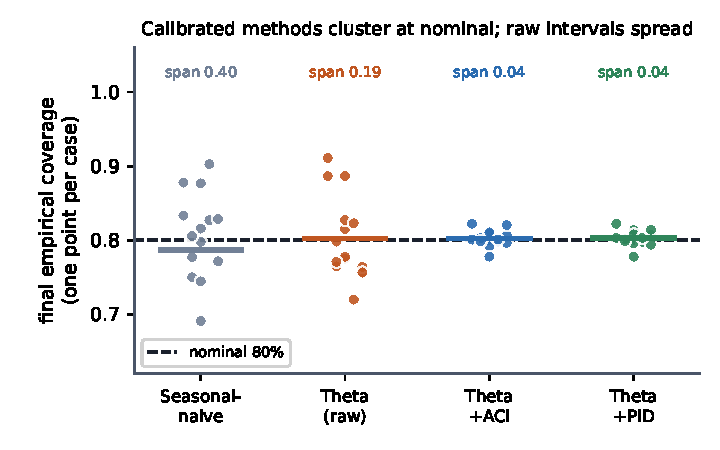
\includegraphics[width=\columnwidth]{fig-coverage-percase.pdf}
\caption{Final empirical coverage, one point per case. The calibrated methods cluster tightly at
the nominal level (across-case span $0.04$) while the raw and naive intervals spread widely (span
$0.19$ and $0.40$). Data: \texttt{streaming.json}.}
\label{fig:percase}
\end{figure}

The headline is Fig.~\ref{fig:summary}. Averaged over the fifteen cases, the raw Theta intervals
miss the nominal $80\%$ target by a mean absolute coverage error of $0.042$ and the seasonal-naive
floor by $0.060$, with worst-case per-case errors of $0.11$ and $0.31$. Wrapping the \emph{same}
Theta point forecaster in ACI or Conformal-PID cuts the mean coverage error to $0.0057$ and
$0.0060$, a sevenfold reduction over raw Theta and tenfold over seasonal-naive. The across-case
view (Fig.~\ref{fig:percase}) shows the same effect as a collapse of dispersion: the final
coverage of the calibrated methods clusters within a $0.04$ span at nominal, while raw Theta
spreads over $0.19$ and seasonal-naive over $0.40$. The point forecast is unchanged (the MASE of
Theta, Theta+ACI and Theta+PID is identical per case); only the interval self-corrects. The effect
is regime-robust: where raw intervals drift most, the calibrators pull the time-averaged coverage
back (intermittent demand raw $0.91\!\to\!$ ACI $0.81$; chaotic Mackey--Glass raw
$0.77\!\to\!0.80$; real UCI electricity raw $0.76\!\to\!0.80$); and on the negative controls
calibration lifts the white-noise coverage from $0.75$ (raw) to $0.79$ while the near-random-walk
control is already at $\approx0.80$ raw and calibration leaves it there ($0.78$), so the harness
does not manufacture skill on unpredictable series, exactly the leakage guard the controls exist to enforce.

% =====================================================================
\section{Discussion and scope}
% =====================================================================

That online conformal calibration keeps streaming intervals near nominal under shift is not by
itself surprising, it is what ACI and Conformal-PID were designed to do. The contribution is that
it is measured under the correct protocol. A stateless rolling-window harness cannot see a
calibrator recover coverage after a regime change, because it does not carry the calibrator's state
across windows; the prequential harness does, and it charges the compute cost that distinguishes a
constant-cost stateful method from a replay wrapper. The negative controls and the identical point
forecasts across raw and calibrated variants rule out the two easy ways such a result could be an
artifact, harness leakage and a point-accuracy confound. Scope: the demonstration uses a Theta base
forecaster because it is a strong classical method that runs live; the calibration is method-agnostic
and wraps any forecaster. The atlas mixes seeded synthetic
regimes with a few real CC-BY series; the synthetic cases isolate regimes and the controls guard
against leakage, but the real-data coverage is reported on a handful of public series, not a large
corpus. Results are shown at horizon one and nominal $80\%$; the harness supports other horizons and
levels. The value we claim is the reusable stateful-streaming harness and the leakage-guarded
measurement, not a new calibrator.

% =====================================================================
\section{Conclusion}
% =====================================================================

We built and released \texttt{preqts}, a prequential streaming evaluation harness for stateful
time-series forecasters with an explicit covariate-arrival policy, embedded in an atlas that pairs
ten diagnostic families with a nineteen-method ladder so the diagnosis explains the leaderboard, and
used it to show, reproducibly and against negative controls, that online conformal calibration
reduces streaming interval coverage error seven-to-tenfold and collapses its across-case spread while
leaving the point forecast unchanged. Evaluating forecasters the way they are deployed, as a stream
with state, is what makes the calibration behavior visible; the harness and the released atlas make
it reproducible.

% =====================================================================
\section*{Data and code availability}
% =====================================================================

{\raggedright
The harness is the open-source package \texttt{preqts} (\url{https://pypi.org/project/preqts/}). The
atlas code, the per-case artifacts (trace, analysis, and streaming trajectories) and the workbench
are at \url{https://github.com/fsantibanezleal/CAOS_RES_ChronoScope} under the MIT license; an
interactive workbench is available at \url{https://chronoscope.fasl-work.com}. Real datasets (UCI
Electricity, Beijing PM2.5, M4 excerpts) are distributed under CC-BY-4.0 with attribution;
streaming artifacts carry aggregate trajectories only. The figures are regenerated
deterministically from these artifacts by
\path{manuscripts/prequential-streaming-conformal/figures/make_figs.py}.\par}

\appendices
\section{The atlas roster}
The ten diagnostic families and their principal methods are listed in Section~\ref{sec:atlas}; each
is a verified implementation with its own theory page (equations, DOIs, and a theme-aware figure) in
the repository \path{docs/analysis/}. The nineteen-method forecast ladder spans classical
(seasonal-naive, SES, Holt, Holt--Winters, Theta), statistical (AutoARIMA, AutoETS, AutoTheta),
gradient-boosted (LightGBM), deep, and stateful foundation models (Chronos, TimesFM). The streaming
roster reported here is the naive floor (seasonal-naive), a strong classical live method (Theta)
with raw intervals, and that same Theta wrapped in ACI and in Conformal-PID; all four are evaluated
by the prequential harness of Section~\ref{sec:harness} at nominal coverage $80\%$, horizon one, and
a per-case warmup of twice the seasonal period floored at 20 steps (20, 24 or 48 across the cases), on all fifteen cases.

% =====================================================================
\begin{thebibliography}{99}
\itemsep 1pt

\bibitem{dawid1984} A.~P. Dawid, ``Present position and potential developments: Some personal views.
Statistical theory. The prequential approach,'' \emph{J. R. Stat. Soc. A}, vol.~147, no.~2,
pp.~278--292, 1984, doi:10.2307/2981683.
\bibitem{gibbs2021} I.~Gibbs and E.~Cand\`es, ``Adaptive conformal inference under distribution
shift,'' in \emph{Adv. Neural Inf. Process. Syst. (NeurIPS)}, 2021, arXiv:2106.00170.
\bibitem{angelopoulos2023} A.~N. Angelopoulos, E.~J. Cand\`es, and R.~J. Tibshirani, ``Conformal PID
control for time series prediction,'' in \emph{Adv. Neural Inf. Process. Syst. (NeurIPS)}, 2023,
arXiv:2307.16895.
\bibitem{shchur2025} O.~Shchur \emph{et al.}, ``fev-bench: A realistic benchmark for time series
forecasting,'' 2025, arXiv:2509.26468.
\bibitem{hyndman2006} R.~J. Hyndman and A.~B. Koehler, ``Another look at measures of forecast
accuracy,'' \emph{Int. J. Forecast.}, vol.~22, no.~4, pp.~679--688, 2006,
doi:10.1016/j.ijforecast.2006.03.001.
\bibitem{makridakis2020} S.~Makridakis, E.~Spiliotis, and V.~Assimakopoulos, ``The M4 competition:
100,000 time series and 61 forecasting methods,'' \emph{Int. J. Forecast.}, vol.~36, no.~1,
pp.~54--74, 2020, doi:10.1016/j.ijforecast.2019.04.014.
\bibitem{gneiting2007} T.~Gneiting and A.~E. Raftery, ``Strictly proper scoring rules, prediction,
and estimation,'' \emph{J. Amer. Statist. Assoc.}, vol.~102, no.~477, pp.~359--378, 2007,
doi:10.1198/016214506000001437.
\bibitem{assimakopoulos2000} V.~Assimakopoulos and K.~Nikolopoulos, ``The theta model: A
decomposition approach to forecasting,'' \emph{Int. J. Forecast.}, vol.~16, no.~4, pp.~521--530,
2000, doi:10.1016/S0169-2070(00)00066-2.
\bibitem{lubba2019} C.~H. Lubba \emph{et al.}, ``catch22: CAnonical Time-series CHaracteristics,''
\emph{Data Min. Knowl. Discov.}, vol.~33, pp.~1821--1852, 2019, doi:10.1007/s10618-019-00647-x.
\bibitem{ansari2024} A.~F. Ansari \emph{et al.}, ``Chronos: Learning the language of time series,''
\emph{Trans. Mach. Learn. Res.}, 2024, arXiv:2403.07815.
\bibitem{das2024} A.~Das, W.~Kong, R.~Sen, and Y.~Zhou, ``A decoder-only foundation model for
time-series forecasting,'' in \emph{Proc. Int. Conf. Mach. Learn. (ICML)}, 2024, arXiv:2310.10688.

\end{thebibliography}

\end{document}
